This lecture is quite short as the second half was spent with a guest lecturer from the Danish energy company Ørsted. I wont cover the guest lecturers talk.

\begin{SCfigure}[][h]
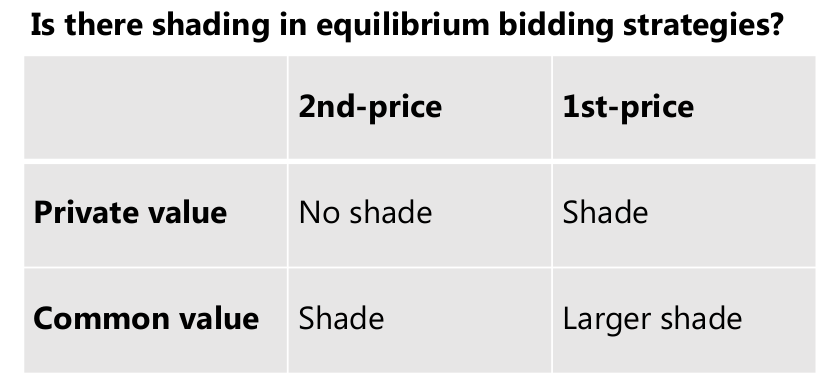
\includegraphics[width=0.4\textwidth]{figures/shadetable.png}    
\caption{\textbf{Auctions overview} Quick overview of the shading behavior of bidders in the auction formats covered so far.}
\end{SCfigure}

\subsection{Revenue linkage principle}
In lecture 4 we saw that it was possible to rank the expected revenues of the three auction formats. This observation leads to a more general formulation about revenues in common value auctions. 

Consider a standard auction in which the highest bidder wins and bidders follow the symmetric equilibrium $\beta^A$. Then from the perspective of bidder 1, let $W^A(z,x)$ be the expected price paid by bidder 1 if he wins by pretending to have signal $z$, while he actually has signal $x$. Examples of $W^A$ are 
\begin{align}
 &   W^I(z,x) = \beta^I(x) \\ 
 &  W^{II}(z,x) = E[\beta^{II}(Y_1)|X_1 = x, Y_1 < z]
\end{align}
The linkage principle states that if $A$ and $B$ are two standard format auctions where the highest bidder wins and \textit{only} he pays a positive amount, and it holds that $W^A(0,0)=W^B(0,0)=0$ and\footnote{where $\partial_2$ indicates we take the derivative w.r.t. the second argument.}
\begin{equation}
    \forall x: \quad \frac{\partial_2 W^A(x,x)}{\partial x} \geq \frac{\partial_2 W^A(x,x)}{\partial x}
\end{equation}
Then the expected revenue in auction $A$ is at least as large as it is in $B$. Intuitively that is if an increase in signal $x$ increases the expected price paid more when playing truthfully, then expected revenue will be higher. We can use this principle to reason about the revenues in different types of common value auctions.  